\section{Analog input output frameworks}
\label{sec:aio-frameworks}

For many users, computers are fairly self-contained systems.  Users
read and write files, using a variety of editors, and share
information between computers via networked connections.  Using
computers to control and monitor arbitrary physical processes is
common in the scientific community and industry, but less so in the
general consumer market.  This means that interfaces between the
digital and analog worlds haven't seen the focused development in the
open source community that more mainstream problem areas have
received.  In this section I'll discuss a few possible options---both
open and proprietary---in the context of my experiment control stack.

\subsection{LabVIEW}
\label{sec:labview}

National Instruments\citep{national-instruments} is a major player in
the experiment control and data aquisition market.  On the hardware
side, they produce a wide range of DAQ cards.  On the software side,
they produce LabVIEW\citep{labview}, a graphical programming language
designed to make writing control and aquisition experiments
straightforward.  Both LabVIEW and NI-DAQmx cards are ubiquitous in
scientific computing; in the four research labs I've worked in over my
career, every lab has used both.  By the time I joined Prof.~Yang's
lab, I'd been using LabVIEW for years, and had become familiar with
its two major limitations: name based linking and a binary file
format.
%
\nomenclature[text ]{DAQ}{Data acquisition.  Although the term only
  refers to input, it is sometimes implicitly extended to include
  signal output as well (for controlling experiments as well as
  measuring results).}

Programming in a graphical language is quite similar to programming in
a textual language.  In both, you reduce complexity by encapsulating
functional subroutines of your process, and then assembling those
subroutines in other, higher-level
subroutines\citep{dijkstra70,wirth74,shneiderman79,hughes89}.  This
means that the application level code can focus on application-level
task (approach the surface, wait for binding, \ldots) without getting
bogged down in the details (increment analog output channel zero in 5
bit steps until analog input channel exceeds 39322 bits).  In textual
languages like C or Python, you can use functions and libraries to
package the functional subroutines.  In LabVIEW, you package the
subroutines in \emph{virtual instruments} (VIs).

\nomenclature[text ]{VI}{Virtual instrument.  LabVIEW's analog to
  functions for encapsulating subroutines.}

The problem comes when you want to update one of your subroutines.
LabVIEW VIs are linked dynamically by VI name\citep{ni-vi-management},
so there was no easy way to swap a new version of the VI into your
application for testing without renaming the subroutine.  With the
Project Explorer (new in LabVIEW 8.0\citep{ni-vi-management}, released
2005), these renames became easier.  However, throughout my time in
the Yang lab, the Windows machines all ran LabVIEW 7.1 (released in
2004).

Because of difficulties with name-based VI linking and the relative
inexperience of many scientists in the maintenance benefits of modular
programming\citep{hilburn93,wilson06b}, LabVIEW code often ends up
without a clean separation between high-level and low-level tasks
(\cref{fig:labview}).  This lack of structure makes it difficult to
reuse existing code to address similar tasks.

\begin{figure}
  \begin{center}
    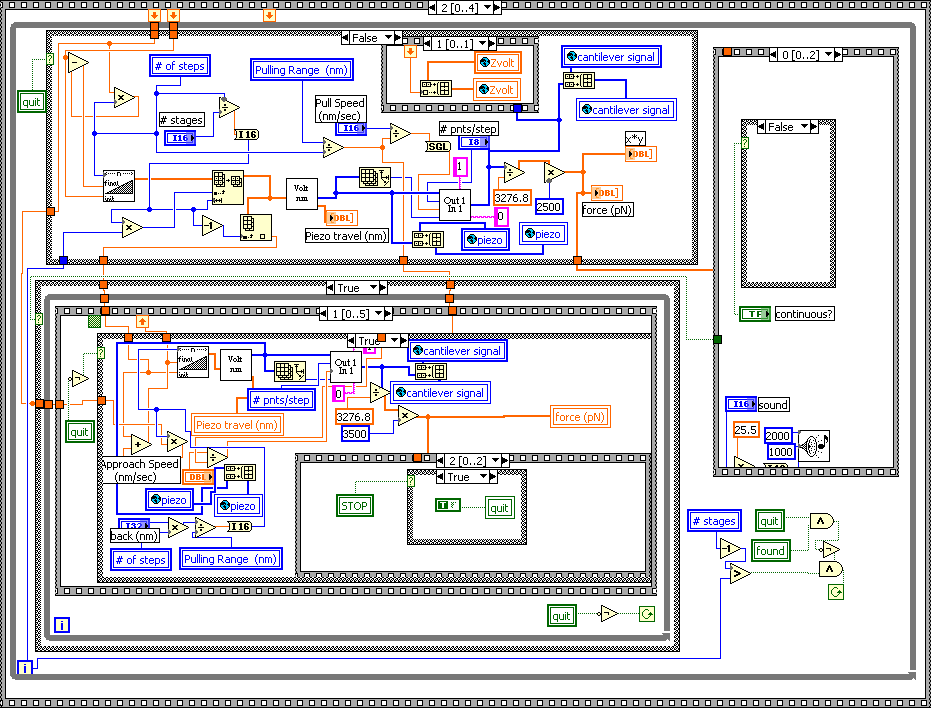
\includegraphics[width=0.8\textwidth]{%
      figures/binary/pulling_chan_1_2d22}
    \caption{An excerpt from the main frame of the LabVIEW stack.
      This frame codes for the velocity-clamped pull phase of a
      push--bind--pull experiment.\label{fig:labview}}
  \end{center}
\end{figure}

The second obstacle to maintaining LabVIEW code is the binary file
format for VIs.  The established method for recording software history
is to use a version control system (VCS), which records versions of
the project in a repository.  Each change to the project is committed
to the repository with some associated metadata (timestamp, committer
name, explanatory message, \ldots).  Users can access this database to
recover earlier versions of the project.  For example, if you find a
bug in your package, you can use your VCS to determine if that bug
affected the data you gathered six months ago.

There are a number of open source version control systems in common
use (Git, Mercurial, and Subversion, \dots), but in order to track and
merge \emph{changes}, they need a way to calculate the difference
between two versions of a given file.  For textual programming
languages, the line-based textual differences used by VCSs work
extremely well, but for binary file formats, performance decreases
drastically.  There are third-party merge tools\citep{ni-merge} for
LabVIEW, but the tools are not officially supported.
%
\nomenclature[text ]{VCS}{Version control system.  A system for
  tracking project development by recording versions of the project in
  a repository.}

While National Instruments seems to put a reasonable amount of effort
into maintaining backwards compatibility, long term archival of binary
formats is still a difficult problem.  For example, our legacy LabVIEW
7.1 installation is no longer compatible with recent LabVIEW releases.
Support for the releases is so low, that without access to the old
LabVIEW release, you may not even be able to determine which version
of LabVIEW your VI corresponds to.  One officially suggested method
for extracting the version from an older VI is\citep{ni-vi-version}:

\begin{quote}
  Open the VI in the earliest version on your computer.  If an error
  occurs, the VI is saved in a later version.  Close the VI and repeat
  this process for the next version of LabVIEW.  The first version
  that opens a VI without any error is the version in which the VI is
  compiled.
\end{quote}

This does not inspire confidence in an ability to extract experiment
control software from VIs after a decade of
archival\citep{ni-vi-upgrade}.

\subsection{NI-DAQmx}
\label{sec:ni-daqmx}

After deciding to avoid LabVIEW, my first attempt at writing an
experiment control framework involved calling National Instrument's
DAQmx library from C\citep{ni-daqmx} (\cref{fig:ni-daqmx}).  I spent
most of 2007 working this framework, using \citetalias{cygwin} as the
development environment.  Inspired by \citetalias{epics}, I built a
message passing server with experiment control and hardware interface
modules connected via sockets.

As the experiment server evolved, I started running into problems.
The overhead of sending all the data through sockets to generic
hardware interface modules was larger than I had na\"{\i}vely
expected.  I also had trouble with multithreaded socket code on
Cygwin, and decided to drop Microsoft Windows altogether in favor of
an open source operating system.

\begin{figure}
  \begin{center}
\begin{minted}{c}
static int set_digital_output_data(DIGITAL_OUTPUT *d, unsigned int data)
{
  d->data = (uInt32) data;
  DAQmxErrChk_struct( Write_WriteDigPort(d->taskHandle, d->data) );
 Error:
  if (d->error != 0) {
    CHK( close_digital_output(d) );
    M_EXIT(FAILURE, "Error in NIDAQ stepper output\n");
  }
  CHK( nsleep(100) );
  PING(1);
  return SUCCESS;
}
\end{minted}
    \caption{An excerpt from the digital output module of my
      experiment server stack.  Most of the C code is error checking
      and tracing macros.  The hardcoded delay time and
      stepper-specific error message are symptoms of my previously
      poor programming practices.  \imint{c}|Write_WriteDigPort| is a
      simplifying wrapper around \imint{c}|DAQmxWriteDigitalU32| from
      the examples bundled with NI-DAQmx.\label{fig:ni-daqmx}}
  \end{center}
\end{figure}

\subsection{Comedi}
\label{sec:comedi}

After transitioning to Linux-based systems, I could no longer use
NI-DAQmx (which only supported Microsoft Windows).  Luckily, the
\citetalias{comedi} project already provided open source driver code
for our DAQ card (an NI-PCI-6052E).  Comedi (from ``Control and
Measurement Device Interface'') is a general purpose library for
interacting with DAQ devices, and supports a wide range of hardware.
When I moved to Comedi, it was a stand-alone kernel module, but since
November 2008 it has been included in the Linux source as a staging
driver.

Comedi development goes back to 2000, so by the time I arrived things
were already pretty stable.  I submitted
\href{http://comedi.org/git?p=comedi/comedi.git;a=commit;h=4284c2266987ad08a26f2758cd09fef06d1ce3cf}{a
  small patch} to support simultaneous analog input/output triggering
on National Instruments cards, and started building my stack.
